\documentclass[../../main.tex]{subfiles}

\begin{document}
\section{Tensor Networks}
    Our goal now is to focus on a subclass of models over $\Sigma^*$. To this end, we analyze \emph{tensor networks}.

    \bigskip
    We denote a tensor \( T_v \) with \( k \) axes of sizes \( D_v = \{d_1, \dots, d_k\} \) as a function
    \[
    T_v : [d_1] \times \dots \times [d_k] \mapsto \mathbb{R} \quad .
    \]
    As a shorthand, we write
    \[
        [D_v] \coloneqq [d_1] \times \dots \times [d_k] \quad .
    \]
    Since indexing is usually clear from context, we treat \( D_v \) as a multiset of axis sizes.

    Given two tensors \( T_u \) and \( T_v \) that share a common axis of size \( d_e \), their contraction over this axis produces a new tensor \( T_C \) with dimension set
    \[
    D_C = (D_u \setminus \{d_e\}) \cup (D_v \setminus \{d_e\}) \quad ,
    \]
    defined as
    \[
    T_C(i) = \sum_{i_e \in [d_e]} T_u(i_{D_u}, i_{e}) \cdot T_v(i_{D_v}, i_{e}) \quad ,
    \]
    where \( i \in [D_C] \). Note that $d_e \not \in D_C$, which is why we explicitly included index $i_{e}$ in the summation.

    \begin{definition}[Tensor Network over \( \Sigma^n \)]
    A \emph{tensor network} \( \mathcal{T} \) over \( \Sigma^n \) is defined by a graph \( G = (V, E) \) with the following structure:
    \begin{itemize}
        \item \( V \) is the set of vertices, where each vertex \( v = (\text{layer}, \text{index}) \in V \) corresponds to a tensor \( T_v \) with axis sizes \( D_v = \{d_1, \dots, d_k\} \). Let \( V_{\text{layer}} \subseteq V \) denote the set of all vertices at a given layer.
        
        \item The input set \( I = (T_{0,1}, \dots, T_{0,n}) \subset V \) consists of tensors each having a single axis of size \( |\Sigma| \). These serve as the one-hot-encoded inputs corresponding to a string \( w \in \Sigma^n \).
        
        \item \( E \subseteq \{\{u, v\} \mid u \in V_l,\, v \in V_{l+1}\} \) is the set of edges. Each edge \( e = \{u, v\} \) represents a shared index of size \( d_e \) between tensors \( T_u \) and \( T_v \), which is summed over during contraction.
        
        \item The usual tensor network constrains: For each vertex \( v \in V \), the degree \( \deg(v) \) must match the number of axes \( |D_v| \), and shared indices must correspond to same axis sizes.
    \end{itemize}

    Once the input tensors are initialized with one-hot encodings derived from a string \( w \in \Sigma^n \), the network computes a scalar output \( \mathcal{T}(w) \). This induces a probability distribution over \( \Sigma^n \) defined by:
    \[
    S_{n, \mathcal{T}}(w) \coloneqq \frac{f(\mathcal{T}(w))}{\sum_{w' \in \Sigma^n} f(\mathcal{T}(w'))} \quad ,
    \]
    where $f: \mathbb{R} \mapsto \mathbb{R}_{\geq 0}$ is any arbitrary function like $f \equiv \exp$.
    \end{definition}

    \begin{figure}[h]
    \center
    \begin{tikzpicture}[
        node distance=1.8cm and 2.5cm,
        every node/.style={draw, circle, minimum size=1.2cm}
    ]

    % Layer 0 (Input) at the bottom
    \node (i1) at (0, 0) {$T_{0,1}$};
    \node (i2) [right=of i1] {$T_{0,2}$};
    \node (i3) [right=of i2] {$T_{0,3}$};

    % Layer 1 (Hidden) in the middle
    \node (h1) [above=of i1] {$T_{1,1}$};
    \node (h2) [above=of i2] {$T_{1,2}$};
    \node (h3) [above=of i3] {$T_{1,3}$};

    % Layer 2 (Output) at the top
    \node (o1) [above=of h2] {$T_{2,1}$};

    % Edges: Input to Hidden
    \draw (i1) -- (h1);
    \draw (i2) -- (h2);
    \draw (i3) -- (h3);

    % Edges: Hidden to Output
    \draw (h1) -- (o1);
    \draw (h2) -- (o1);
    \draw (h3) -- (o1);

    % Layer labels
    \node[draw=none, below=0.2cm of i2] {Input Layer};
    \end{tikzpicture}
    \caption{A basic tensor network over $\Sigma^3$.}
    \end{figure}


    \bigskip
    \begin{definition}[Normalized and Non-Negative Tensor Networks]
        Let $\mathcal{T}$ be a tensor network over $\Sigma^n$ with scalar output $\mathcal{T}(w)$ for each $w \in \Sigma^n$. Define the total mass of the network as
        \[
            |\mathcal{T}| \coloneqq \sum_{w \in \Sigma^n} \mathcal{T}(w) \quad .
        \]
        We say $\mathcal{T}$ is \emph{normalized} iff $|\mathcal{T}| = 1$.

        Furthermore, a tensor network is said to be \emph{non-negative} iff for all $w \in \Sigma^n$ we have $\mathcal{T}(w) \geq 0$.
    \end{definition}

    \begin{remark}
        We can enforce all tensor networks of our model space to be non-negative by only allowing for non-negative tensors in the networks.
    \end{remark}

    \begin{definition}[Normalization of Tensor Networks]
        Let $\mathcal{T}$ be a tensor network over $\Sigma^n$, and let $H \coloneqq V \setminus I$ be the set of non-input tensors, and define $|H|$ as its cardinality. The \emph{induced normalized tensor network} $\dfrac{\mathcal{T}}{|\mathcal{T}|}$ is the same network as $\mathcal{T}$, but each entry of each tensor in $H$ is scaled by the factor $\dfrac{1}{\sqrt[|H|]{|\mathcal{T}|}}$.
    \end{definition}


    \begin{lemma}
        \label{lemma:normalized_tensor_networks}
        Let $J \subseteq [n]$ and let $\mathcal{T}$ be a tensor network over $\Sigma^n$. Define a modified network $\mathcal{T}_J$ where for all $j \in J$, the input tensor $T_{0,j}$ is initialized to the all-ones vector (i.e., $\mathbf{1} \in \mathbb{R}^{|\Sigma|}$). Then for any $w \in \Sigma^{[n] \setminus J}$:
        \[
            \sum_{w_J \in \Sigma^{|J|}} \mathcal{T}(w_J, w) = \mathcal{T}_J(w) \quad .
        \]
    \end{lemma}
    \begin{proof}
    We proceed by induction on the size of the subset \( J \subseteq [n] \).

    \textbf{Base case:} \( |J| = 0 \).  
    Then \( J = \emptyset \), so \( \mathcal{T}_J = \mathcal{T} \), and the sum over \( w_J \in \Sigma^{|J|} \) is a sum over a singleton (the empty word), yielding:
    \[
        \sum_{w_J \in \Sigma^0} \mathcal{T}(w_J, w) = \mathcal{T}(w),
    \]
    and since \( \mathcal{T}_J(w) = \mathcal{T}(w) \), the base case holds.

    \textbf{Inductive step:}  
    Assume the lemma holds for all subsets of size \( k \), and let \( J \subseteq [n] \) with \( |J| = k+1 \). Pick any \( j_0 \in J \), and define \( J' = J \setminus \{j_0\} \), which has size \( k \). By the inductive hypothesis, for any \( w \in \Sigma^{[n] \setminus J} \), we have:
    \[
        \sum_{w_{J'} \in \Sigma^{k}} \mathcal{T}(w_{J'}, w, w_{j_0}) = \mathcal{T}_{J'}(w, w_{j_0}) \quad ,
    \]
    where \( w_{j_0} \in \Sigma \) varies over its values.

    Now consider the sum over all \( w_J \in \Sigma^{k+1} \), which we write as:
    \[
        \sum_{w_{J'} \in \Sigma^k} \sum_{w_{j_0} \in \Sigma} \mathcal{T}(w_{J'}, w_{j_0}, w) \quad .
    \]
    By the inductive hypothesis, this equals:
    \[
        \sum_{w_{j_0} \in \Sigma} \mathcal{T}_{J'}(w_{j_0}, w) \quad .
    \]
    Observe that in \( \mathcal{T}_{J'} \), the input tensor at position \( j_0 \) is still initialized to a one-hot vector, while the inputs at \( J' \) have been replaced with the all-ones vector.

    Now, note that the inner sum over \( w_{j_0} \) is equivalent to replacing the input at \( j_0 \) with the all-ones vector, since the sum represents a sum over vector dot products of vector $\bm{v}_{w_{j_0}} \coloneqq \mathcal{T}_{J'}(w_{j_0}, w)$ with one-hot encoded vectors. It follows from linearity that we can factor out $\bm{v}$, and the sum of the one-hot encoded vector yields the all-ones vector. Thus:
    \[
        \sum_{w_{j_0} \in \Sigma} \mathcal{T}_{J'}(w_{j_0}, w) = \mathcal{T}_J(w) \quad .
    \]
    Hence, by induction, the lemma holds for all subsets \( J \subseteq [n] \).

    \end{proof}

    \begin{corollary}
        Let $\mathcal{T}$ be a tensor network over $\Sigma^n$, and let $\mathcal{T}_{[n]}$ be the network where all input tensors are initialized to the all-ones vector. Then:
        \[
            \mathcal{T} \text{ is normalized} \iff \mathcal{T}_{[n]} = 1 \quad ,
        \]
        i.e., the total contraction of the network with all-one input tensors equals 1.
    \end{corollary}

    \begin{lemma}
        Let $\mathcal{T}$ be a tensor network over $\Sigma^n$. The induced normalized tensor network $\frac{\mathcal{T}}{|\mathcal{T}|}$ is indeed normalized, and if additionally $\mathcal{T}$ is non-negative and $f \equiv \text{id}$, we have for all $w \in \Sigma^n$:
        \[
            S_{n, \mathcal{T}}(w) = S_{n, \frac{\mathcal{T}}{|\mathcal{T}|}}(w) \quad .
        \]
    \end{lemma}
    \begin{proof}
        Let $H$ be the set of non-input tensors in $\mathcal{T}$, and let $|H| = m$. In the induced normalized network, every tensor in $H$ is scaled by a factor $\alpha = \dfrac{1}{\sqrt[m]{|\mathcal{T}|}}$. Since the final output $\mathcal{T}(w)$ is a multilinear contraction over the tensors, this means the scalar output for any $w \in \Sigma^n$ becomes:
        \[
            \left( \prod_{v \in H} \alpha \right) \cdot \mathcal{T}(w) = \alpha^m \cdot \mathcal{T}(w) = \frac{1}{|\mathcal{T}|} \cdot \mathcal{T}(w) \quad .
        \]
        Hence,
        \[
            \left(\frac{\mathcal{T}}{|\mathcal{T}|}\right)(w) = \frac{\mathcal{T}(w)}{|\mathcal{T}|} \quad .
        \]

        Summing over all \( w \in \Sigma^n \),
        \[
            \left| \frac{\mathcal{T}}{|\mathcal{T}|} \right| = \sum_{w \in \Sigma^n} \frac{\mathcal{T}(w)}{|\mathcal{T}|} = \frac{1}{|\mathcal{T}|} \sum_{w \in \Sigma^n} \mathcal{T}(w) = \frac{|\mathcal{T}|}{|\mathcal{T}|} = 1 \quad .
        \]

        Moreover, since the normalization rescales all outputs by the same constant, the ratio of the terms to the total sum remains unchanged:
        \[
            S_{n, \frac{\mathcal{T}}{|\mathcal{T}|}}(w) = \frac{\left( \frac{\mathcal{T}(w)}{|\mathcal{T}|} \right)}{\sum_{w' \in \Sigma^n} \left( \frac{\mathcal{T}(w')}{|\mathcal{T}|} \right)} = \frac{\mathcal{T}(w)}{|\mathcal{T}|} \cdot \frac{1}{1} = S_{n, \mathcal{T}}(w) \quad .
        \]

        This completes the proof.
    \end{proof}



    One might ask whether our definition for tensor networks is bit restrictive, as it only allows for contraction over \emph{pairs} of tensors. But what if we wanted to contract, say, three tensors at once over a common index?

    \begin{proposition}
        \label{proposition:contracting_over_shared_index}
        Let $V' \subseteq V$ be a set of tensors in a tensor network, each containing an axis of dimension $d$ labeled by a shared index $i$. Contracting all tensors in $V'$ over the shared index $i$ is equivalent to contracting each tensor individually with a single tensor 
        \[
        \delta_{|V'|} : [d]^{|V'|} \mapsto \mathbb{R}_{\geq 0}
        \]
        defined by
        \[
        \delta_{|V'|}(i_1, \dots, i_{|V'|}) = 
        \begin{cases}
        1 & \text{if } i_1 = \dots = i_{|V'|} \ , \\
        0 & \text{otherwise.}
        \end{cases}
        \quad .
        \]
        That is, a full contraction over a shared index can be implemented by introducing a single copy tensor connected to each tensor in $V'$.
    \end{proposition}

    \begin{proof}
    Each tensor $T_v$ for $v \in V'$ has an index \( i \in [d] \) corresponding to the shared axis. The contraction over this index is defined by summing over the common value of \( i \) across all tensors:
    \[
    \sum_{i=1}^d \prod_{v \in V'} T_v(\dots, i, \dots) \quad .
    \]

    Now consider a new tensor \( \delta_{|V'|} \) of order \( |V'| \), defined as 1 if all indices are equal and 0 otherwise. Let each tensor \( T_v \) maintain its original indices, but connect to \( \delta_{|V'|} \) via the position corresponding to \( v \).

    The contraction over this shared structure gives:
    \[
    \sum_{i_1, \dots, i_{|V'|}} \left( \prod_{v \in V'} T_v(\dots, i_v, \dots) \right) \delta_{|V'|}(i_1, \dots, i_{|V'|}) \quad .
    \]

    By definition of \( \delta_{|V'|} \), this enforces \( i_1 = \dots = i_{|V'|} \), reducing the above to:
    \[
    \sum_{i=1}^d \prod_{v \in V'} T_v(\dots, i, \dots) \quad ,
    \]
    which is exactly the original contraction. Hence, the two constructions are equivalent.
    \end{proof}

    \begin{figure}[h]
        \center
        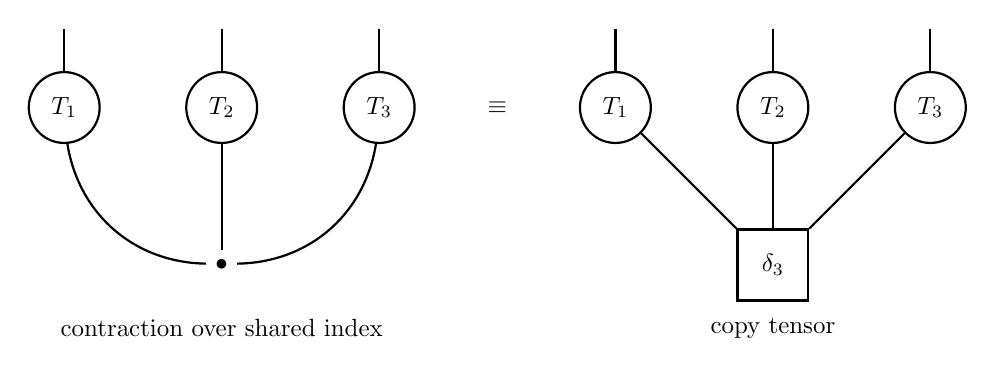
\begin{tikzpicture}[thick, scale=1.0, every node/.style={scale=0.9}]
            % Left side - shared index (hyperedge)
            \node[draw, circle, minimum size=1cm] (L1) at (-4, 0) {$T_1$};
            \node[draw, circle, minimum size=1cm] (L2) at (-2, 0) {$T_2$};
            \node[draw, circle, minimum size=1cm] (L3) at (0, 0) {$T_3$};
            \node (H) at (-2, -2) {$\bullet$};
            \node at (-2, -2.8) {contraction over shared index};

            % Curved edges to show shared index
            \draw[bend right=40] (L1) to (H);
            \draw (L2) to (H);
            \draw[bend left=40] (L3) to (H);


            \node at (1.5, 0) {$\equiv$};

            % Right side - copy tensor
            \node[draw, circle, minimum size=1cm] (R1) at (3, 0) {$T_1$};
            \node[draw, circle, minimum size=1cm] (R2) at (5, 0) {$T_2$};
            \node[draw, circle, minimum size=1cm] (R3) at (7, 0) {$T_3$};

            \node[draw, rectangle, minimum size=1cm, inner sep=0pt] (delta) at (5, -2) {$\delta_3$};

            % Connections to copy tensor
            \draw[-] (delta) -- (R1);
            \draw[-] (delta) -- (R2);
            \draw[-] (delta) -- (R3);

            \node at (5, -2.8) {copy tensor};

            % Optional: inputs
            \draw[-] (L1) -- (-4, 1);
            \draw[-] (L2) -- (-2, 1);
            \draw[-] (L3) -- (0, 1);
            \draw[-] (R1) -- (3, 1);
            \draw[-] (R2) -- (5, 1);
            \draw[-] (R3) -- (7, 1);
        \end{tikzpicture}
        \caption{Contracting multiple tensors over one shared index is equivalent to contracting them individually with a single copy tensor.}
    \end{figure}

    \subsection{Reshaping a Tensor by a Partition (Matricization)}
    A tensor network defines a probability tensor with $|\Sigma|^n$ entries. However, we can reshape this tensor by grouping together some axes. To this end, we first define a \emph{partition}:

    \begin{definition}
        Let $I = \{1, 2, \dots, n\}$ be a set of indices. A \emph{partition} of $I$ is a collection of non-empty, pairwise disjoint subsets $\{I_1, I_2, \dots, I_k\}$ of $I$ whose union is $I$. That is:
        \begin{enumerate}
            \item $I_j \neq \emptyset$ for all $j \in \{1, \dots, k\}$
            \item $I_j \cap I_l = \emptyset$ for all $j \neq l$
            \item $\bigcup_{j=1}^k I_j = I$
        \end{enumerate}
        The subsets $I_j$ are called the \emph{parts} of the partition.
    \end{definition}

    In the context of a tensor with $n$ axes, a partition of its indices allows for grouping these axes together, effectively reshaping the tensor. Partitions with two parts allows us to represent a tensor by a matrix. To this end, we use the notation
    % $\llbracket T \rrbracket_{A,B}$
    $[[T]]_{A,B}$
    to represent the reshaping of a tensor $T$ into a matrix based on the partition $\{A,B\}$. This operation, also known as \emph{matricization}, \emph{unfolding}, or \emph{flattening}, relies on partitioning the tensor's indices into two distinct sets, one for the rows and one for the columns of the new matrix. Formally:

    \begin{definition}[Tensor Matricization]
    Let $T$ be an order-$k$ tensor with indices in the set $I = \{1, 2, \dots, k\}$, and corresponding dimensions $d_1, d_2, \dots, d_k$. Let $\{A, B\}$ be a bipartition of $I$, such that $A \cup B = I$ and $A \cap B = \emptyset$. Let $A = \{a_1, \dots, a_{|A|}\}$ and $B = \{b_1, \dots, b_{|B|}\}$ be ordered sets of indices.

    The matricization of $T$ with respect to the partition $\{A, B\}$ is the matrix $M = $ of size $D_A \times D_B$, where:
    \begin{itemize}
        \item The number of rows is $D_A = \prod_{j \in A} d_j$.
        \item The number of columns is $D_B = \prod_{j \in B} d_j$.
    \end{itemize}
    An element $T_{i_1, i_2, \dots, i_k}$ of the tensor is mapped to an element $M_{\alpha, \beta}$ of the matrix, where the row index $\alpha$ and column index $\beta$ are "super-indices" formed from the indices in $A$ and $B$, respectively. Assuming a lexicographical ordering, the mapping is given by:
    \begin{align*}
        \alpha &= 1 + \sum_{j=1}^{|A|} (i_{a_j} - 1) \left( \prod_{l=j+1}^{|A|} d_{a_l} \right) \\
        \beta &= 1 + \sum_{j=1}^{|B|} (i_{b_j} - 1) \left( \prod_{l=j+1}^{|B|} d_{b_l} \right)
    \end{align*}
    \end{definition}

    \subsubsection{An Upper Bound for the Rank of Matrices in Tensor Networks}
    We can analyze these matrices, which depend on the partition $\{A, B\}$, of our tensor network. When picturing it as a graph, we can separate the states in $A$ from the states in $B$ with a cut. Metaphorically, we see that $A$ and $B$ \emph{communicate} over this cut. Hence, we might assume that if the associated bond dimensions are small, so is the mutual information between the two sets. In fact, this intuition is backed up by mathematical evidence:

    \begin{theorem}
    \label{theorem:min_cut_caps_rank}
Let $\mathcal{T}$ be a tensor represented by a tensor network over a set of physical indices $\mathcal{I} = \{i_1, \dots, i_N\}$. For any bipartition of these indices into sets $\mathcal{I}_A$ and $\mathcal{I}_B$, which induces a cut through a set of internal bonds $E_{cut} = \{e_1, \dots, e_c\}$ with dimensions $\{D_1, \dots, D_c\}$, the rank of the reshaped matrix $M$ corresponding to this partition is bounded by:
$$
\text{rank}(M) \le \prod_{k=1}^{c} D_k
$$
\end{theorem}

\begin{proof}
A tensor network represents a tensor $\mathcal{T}$ by contracting a set of smaller tensors. Let's visualize a generic tensor network. A bipartition of the physical indices $(\mathcal{I}_A, \mathcal{I}_B)$ divides the graph of the network into two subgraphs.

\begin{figure}[h!]
\centering
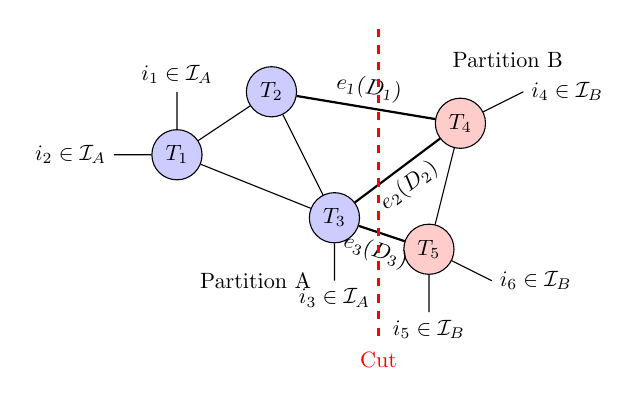
\begin{tikzpicture}[scale=0.8, every node/.style={transform shape}]
    % Nodes (tensors)
    \node[circle, draw, fill=blue!20] (T1) at (0,2) {$T_1$};
    \node[circle, draw, fill=blue!20] (T2) at (1.5,3) {$T_2$};
    \node[circle, draw, fill=blue!20] (T3) at (2.5,1) {$T_3$};
    \node[circle, draw, fill=red!20] (T4) at (4.5,2.5) {$T_4$};
    \node[circle, draw, fill=red!20] (T5) at (4,0.5) {$T_5$};

    % Physical indices
    \draw (T1) -- ++(0,1) node[above] {$i_1 \in \mathcal{I}_A$};
    \draw (T1) -- ++(-1,0) node[left] {$i_2 \in \mathcal{I}_A$};
    \draw (T3) -- ++(0,-1) node[below] {$i_3 \in \mathcal{I}_A$};
    \draw (T4) -- ++(1,0.5) node[right] {$i_4 \in \mathcal{I}_B$};
    \draw (T5) -- ++(0,-1) node[below] {$i_5 \in \mathcal{I}_B$};
    \draw (T5) -- ++(1,-0.5) node[right] {$i_6 \in \mathcal{I}_B$};

    % Internal bonds
    \draw (T1) -- (T2);
    \draw (T1) -- (T3);
    \draw (T3) -- (T2);
    \draw (T4) -- (T5);
    
    % Cut bonds
    \draw[thick] (T2) -- (T4) node[midway, above, sloped] {$e_1 (D_1)$};
    \draw[thick] (T3) -- (T4) node[midway, below, sloped] {$e_2 (D_2)$};
    \draw[thick] (T3) -- (T5) node[midway, below, sloped] {$e_3 (D_3)$};

    % The cut
    \draw[dashed, red, thick, rounded corners] (3.2, 4) -- (3.2, -1) node[below] {Cut};
    
    \node at (1.25, 0) {Partition A};
    \node at (5.25, 3.5) {Partition B};
\end{tikzpicture}
\caption{A generic tensor network with a cut partitioning the physical indices into $\mathcal{I}_A$ (blue) and $\mathcal{I}_B$ (red). The cut crosses bonds $e_1, e_2, e_3$.}
\end{figure}

We can group all tensors on the left of the cut (Partition A) and contract their internal bonds among themselves. This results in a single, large tensor, which we call $U$. The indices of $U$ are the physical indices in $\mathcal{I}_A$ and the cut bond indices $\{e_1, \dots, e_c\}$. Likewise, we contract all tensors in Partition B to form a tensor $V$, with indices from $\mathcal{I}_B$ and $\{e_1, \dots, e_c\}$.

\begin{figure}[h!]
\centering
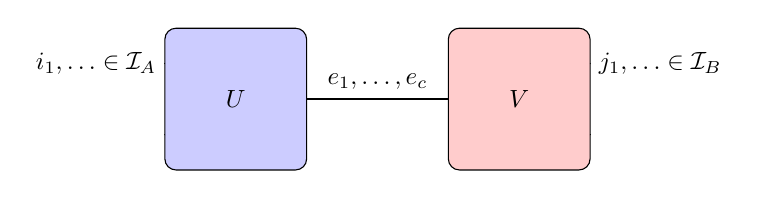
\begin{tikzpicture}[scale=0.9, every node/.style={transform shape}]
    % Grouped tensor U
    \node[draw, rounded corners, fill=blue!20, minimum height=2cm, minimum width=2cm] (U) at (0,0) {$U$};
    \draw (U) -- ++(-1, 0.5) node[left] {$i_1, \dots \in \mathcal{I}_A$};
    \draw (U) -- ++(-1, -0.5);

    % Grouped tensor V
    \node[draw, rounded corners, fill=red!20, minimum height=2cm, minimum width=2cm] (V) at (4,0) {$V$};
    \draw (V) -- ++(1, 0.5) node[right] {$j_1, \dots \in \mathcal{I}_B$};
    \draw (V) -- ++(1, -0.5);

    % Cut bonds connecting U and V
    \draw[thick] (U) -- (V) node[midway, above] {$e_1, \dots, e_c$};
\end{tikzpicture}
\caption{Contracting the subgraphs results in two tensors, $U$ and $V$, connected by the cut bonds.}
\end{figure}

The original tensor $\mathcal{T}$ is recovered by contracting $U$ and $V$ over the cut indices. Now, we reshape $U$ and $V$ into matrices. Let $\alpha$ be a multi-index that combines all cut indices $\{e_1, \dots, e_c\}$. The dimension of this multi-index is $D_{cut} = \prod_{k=1}^{c} D_k$.
Let $I_A$ be the multi-index for all physical indices in $\mathcal{I}_A$.
Let $I_B$ be the multi-index for all physical indices in $\mathcal{I}_B$.

We reshape the tensor $U$ into a matrix $\mathbf{U}$ of size $(\dim(I_A) \times D_{cut})$ where the rows are indexed by $I_A$ and the columns by $\alpha$.
We reshape the tensor $V$ into a matrix $\mathbf{V}$ of size $(D_{cut} \times \dim(I_B))$ where the rows are indexed by $\alpha$ and the columns by $I_B$.

The reshaped tensor matrix $M$ (with rows $I_A$ and columns $I_B$) is exactly the matrix product of $\mathbf{U}$ and $\mathbf{V}$:
$$ M = \mathbf{U} \cdot \mathbf{V} $$

\begin{figure}[h!]
\centering
\begin{tikzpicture}
    % Matrix U
    \node[draw, fill=blue!20, minimum width=1.5cm, minimum height=2.5cm, label=below:$\mathbf{U}$] (U_mat) at (0,0) {};
    \node[left=0.1 of U_mat] (IA) {$\dim(I_A)$};
    \node[above=0.1 of U_mat] (Dcut_U) {$D_{cut}$};
    
    % Equals sign
    \node (=) at (3,0) {$=$};
    
    % Matrix multiplication
    \node[draw, fill=blue!20, minimum width=1.5cm, minimum height=2.5cm, label=below:$\mathbf{U}$] (U_prod) at (1.5,0) {};
    \node[left=0.1 of U_prod] {$\dim(I_A)$};
    \node[above=0.1 of U_prod] {$D_{cut}$};
    
    \node[draw, fill=red!20, minimum width=2.5cm, minimum height=1.5cm, label=below:$\mathbf{V}$] (V_prod) at (4.25, 0) {};
    \node[left=0.1 of V_prod] {$D_{cut}$};
    \node[above=0.1 of V_prod] {$\dim(I_B)$};
    
    % Matrix M
    \node[draw, minimum width=2.5cm, minimum height=2.5cm, label=below:$M$] (M_mat) at (-2,0) {};
    \node[left=0.1 of M_mat] {$\dim(I_A)$};
    \node[above=0.1 of M_mat] {$\dim(I_B)$};

    % Arrows
    \draw[->, thick] (U_prod.east) -- (V_prod.west) node[midway, below, yshift=-2mm] {Contraction over $D_{cut}$};
\end{tikzpicture}
\caption{The matrix $M$ is a product of matrices $\mathbf{U}$ and $\mathbf{V}$, with inner dimension $D_{cut}$.}
\end{figure}

A fundamental property of linear algebra states that the rank of a product of matrices is at most the minimum of their individual ranks:
$$ \text{rank}(M) = \text{rank}(\mathbf{U} \cdot \mathbf{V}) \le \min(\text{rank}(\mathbf{U}), \text{rank}(\mathbf{V})) $$
The rank of a matrix is also bounded by its dimensions. For $\mathbf{U}$ and $\mathbf{V}$, we have:
$$ \text{rank}(\mathbf{U}) \le \min(\dim(I_A), D_{cut}) \le D_{cut} $$
$$ \text{rank}(\mathbf{V}) \le \min(D_{cut}, \dim(I_B)) \le D_{cut} $$
Therefore, the rank of $M$ is bounded by the total dimension of the cut:
$$ \text{rank}(M) \le D_{cut} = \prod_{k=1}^{c} D_k $$
This completes the proof.
\end{proof}
\end{document}